%
% fourier.tex -- oszillationsphänomene insbesondere Milankowitsch-Zyklern
%
% (c) 2018 Prof Dr Andreas Müller, Hochschule Rapperswil
%
\chapter{Fourier-Analysis\label{chapter:fourier}}
\lhead{Fourier-Analysis}
\rhead{ }
Im Kapitel~\ref{chapter:wetter und klima} wurde gezeigt, dass einige der
Einflüsse
auf das Klimasystem periodisch sind mit einer Periode, die vergleichbar
oder grösser ist als die bei der Definition des Begriffes Klima üblicherweise
verwendeten Mittelungszeitspanne.
Diese Anregungen führen daher zu periodischen Klimaschwankungen.
Die Fourier-Analysis ermögilcht, solche periodischen Einflüsse in
einem Signal zu erkennen und sie von anderen Phänomenen zu trennen.

%
% periodisch.tex -- periodische Funktionen
%
% (c) 2018 Prof Dr Andreas Müller, Hochschule Rapperswil
%
\section{Periodische Funktionen}
Das ursprüngliche Budyko-Modell modelliert die Jahresmitteltemperatur,
ignoriert also die Temperaturentwicklung der Temperatur im Laufe des
Jahres.
Damit ist es aber zum Beispiel nicht möglich, das Einsetzen von
Eiszeiten zu modellieren.
Die jährlich
auf die Erde eingetrahlte Energie ist unabhängig von der Neigung der
Erdachse.
Ein Modell, welches den Zusammenhang zwischen Eiszeiten und der
Achsneigung modellieren soll, muss also die periodischen Schwankungen
der Einstrahlung der Sonne auf jede Erd-Halbkugel berücksichtigen.

Ein geeignetes Modell wird also nicht mehr autonom sein, sondern auf der
rechten Seite der Differentialgleichung
\[
\frac{dx}{dt} = f(x,t)
\]
eine Funktion $f(x,t)$ haben, die nun auch von der Zeit $t$ abhängt
und periodisch in $t$ mit Periode $T$ ist.
Dies bedeutet $f(x,t+T)=f(x,t)$ für beliebige Vektoren $x$ und 
Zeiten $t$.
Die Periode muss nicht unbedingt genau ein Jahr sein, es sind auch
Vielfache eines Jahres denkbar.

Man kann natürlich nicht mehr erwarten, dass es eine zeitunabhängige
Gleichgewichtslösung gibt.
Vielmehr erwarten wir statt konstanter Gleichgewichtslösungen 
periodische Lösungen mit der gleichen Periode $T$, dass also
$x(t+T)=x(t)$.

\subsection{Fourierreihen}
Die Funktionen
\begin{equation}
1,\quad
\cos \frac{2\pi kt}{T},\quad
\sin \frac{2\pi kt}{T},\qquad k\in \mathbb N
\label{skript:periodisch:fourierbasis}
\end{equation}
sind alle periodisch mit Periode $T$, aber auch eine beliebige
Linearkombination
\begin{equation}
f(t)
=
a_0  +\sum_{k=1}^\infty\biggl(
a_k \cos \frac{2\pi kt}{T} + b_k\sin\frac{2\pi kt}{T}
\biggr),
\label{skript:periodisch:fourierreihe}
\end{equation}
ein sogenanntes trigonometrisches Polynom, hat diese Eigenschaft.
Damit lässt sich eine grosse Vielfalt von $2\pi$-periodischen
Funktionen wiedergeben.

Es war die bedeutende Erkenntnis von Joseph Fourier, dass bis auf ein
\index{Fourier, Joseph}%
paar technische Bedingungen, welche die Konvergenz der Funktionenreihe
\eqref{skript:periodisch:fourierreihe}
sicherstellen sollen, jede periodische Funktion $f(t)$ 
als Reihe von Vielfachen der Funktionen
\eqref{skript:periodisch:fourierbasis}
in der Form
\eqref{skript:periodisch:fourierreihe}
dargestellt werden kann.
Diese Bedingungen sind für stetige Funktionen immer erfüllt.
Die Berechnung der Koeffizienten $a_0,a_1,a_2,\dots$ und $b_1,b_2,b_3,\dots$
erfolgt mit Hilfe von Fourier-Integralen, deren Theorie wir hier weiter
nicht entwickeln wollen, wir kommen darauf in
Abschnitt~\ref{subsection:fourier:stetig} zurück.

Für unsere Zwecke ist die vollständige Theorie der Fourier-Reihen nicht
notwendig, denn die Daten, an die wir unsere Klimamodelle anpassen
müssen, stellen bestenfalls diskrete Approximationen von stetigen
Funktionen dar.
Wir müssen die allgemeine Fourier-Theorie daher spezialisieren auf diese
diskrete Situation.

\subsection{Diskrete Fourierreihen}
Wir wollen im Folgenden periodische diskrete Funktionen möglichst gut
approximieren.
Die Diskretisation wird charakterisiert durch die Anzahl
$N$ der bekannten Werte im Periodeninterval $[0,2\pi)$.

\subsubsection{Diskretisation}
Gegeben sind also die Werte $y_j$ einer $2\pi$-periodischen Funktion
$f(t)$ an den äquidistanten Stellen $t_j=2\pi j/N$ mit
$1\le j \le N$.
Da $f(t)$ eine $2\pi$-periodische Funktion ist, folgt
\[
y_j = f(t_j) = f(t_j+2\pi) = f(t_{j+N}).
\]
Wir erweitern daher die Notation für $y$ und setzen
\[
y_j = y_{r(j)},
\]
wobei $r(j)$ der Rest von $j$ bei Teilung durch $N$ steht.
Insbesondere ist $y_0=y_N$, die Folge $y_j$ ist $N$-periodisch als
Folge von reellen Zahlen.

\subsubsection{Trigonometrische Polynome}
Als Basis für die Darstellung der Funktion $f(t)$ verwenden wir
die bekanntermassen
$2\pi$-periodischen Funktionen 
\begin{equation}
1,\quad \cos kt\quad\text{und}\quad \sin kt,\qquad k\in\mathbb N.
\end{equation}
Die Funktion $f(t)$ soll also geschrieben werden als sogenanntes 
{\em trigonometrisches Polynom}
\index{trigonometrisches Polynom}%
\begin{equation}
f(t)
=
a_0 + \sum_{k=1}^n \bigl(a_k \cos kt + b_k\sin kt).
\label{skript:fourier:rekonstruktion}
\end{equation}
Ein Koeffizient $b_0$ ist nicht sinnvoll, weil die dazugehörige Basisfunktion
$\sin 0t =0$ ist.
Die Funktion $f(t)$ soll die Werte $y_j$
möglichst gut wiedergeben, es soll also wenn möglich $f(t_j) = y_j$ sein.

Zur Bestimmung der Koeffizienten $a_0$, $a_k$ und $b_k$ stehen genau
die $N$ Bedingungen
\begin{equation}
f(t_j)=y_j
\label{skript:periodisch:fourierbedingungen}
\end{equation}
zur Verfügung.
Die Gleichungen \eqref{skript:periodisch:fourierbedingungen} sind
lineare Gleichungen für die Unbekannten $a_k$ und $b_k$ mit
$\cos kt_j$ und $\sin kt_j$ als Koeffizienten.
Sie können daher höchstens $N$ der Koeffizienten $a_k$ und $b_k$
bestimmen.
Dieses Problem wird im nächsten Abschnitt gelöst.


%
% fourierkoef.tex -- Bestimmung der Fourier-Koeffizienten
%
% (c) 2018 Prof Dr Andreas Müller, Hochschule Rapperswil
%
\section{Fourier-Koeffizienten}
\rhead{Fourier-Koeffizienten}
In diesem Abschnitt bestimmen wir die Fourierkoeffizienten für ein
trigonometrisches Polynom der Form
\begin{equation}
p_n(t)
=
a_0 + \sum_{k=1}^{n-1} a_k\cos kt + \sum_{k=1}^{n-1} b_k\sin kt + a_n\cos nt,
\label{skript:fourier:ansatz}
\end{equation}
derart, dass die Werte
\begin{equation}
y_j \quad\text{zu den Zeitpunkten}\quad t_j=2\pi\frac{j}{N},\qquad 1\le j< N
\label{skript:fourier:gleichungen}
\end{equation}
möglichst genau die Funktionswerte $p_n(t_j)$ reproduzieren.

Im Ansatz~\eqref{skript:fourier:ansatz} für $p_n(t)$ finden wir
genau $2n$ zu bestimmende Koeffizienten, nämlich $a_0$,
$n$ Koeffizienten $a_k$ mit $k=1,\dots,n$
und $n-1$ Koeffizienten $b_k$ mit $k=1,\dots,n-1$.
Mit $N$ Datenpunkten $y_j$ haben wir genau die $N$ Bedingungen
$p_n(t_j)=y_j$, um diese Koeffizienten zu bestimmen.
Die Bedingungen $p_n(t_j)=y_j$ sind $N$ lineare Gleichungen für die
$2n$ Koeffizienten, sie dürften sich also genau dann exakt lösen
lassen, wenn $N=2n$, wenn also die Zahl der Datenpunkte gerade ist.

Für $N<2n$ haben wir weniger Gleichungen als Koeffizienten, es ist
also unmöglich, die Koeffizienten ohne zusätzliche Annahmen zu bestimmen.
Das Problem ist also nur dann überhaupt lösbar, wenn $N\ge 2n$ ist.
Für $N>2n$ haben wir zu viele Daten, wir können nicht erwarten, dass
das Gleichungssystem $p_n(t_j)=y_j$ überhaupt eine Lösung hat.
Im optimalen Fall, für $N=2n$ sollte es möglich sein, die Koeffizienten so
zu bestimmen, dass die Funktionswerte $y_j$ exakt reproduziert werden.

\subsection{Least Squares}
Für $N>2n$ können wir nicht erwarten, dass der Ansatz
\eqref{skript:fourier:ansatz} die Daten exakt reproduzieren kann,
wir müssen uns also mit einer Näherungslösung begnügen.
Wir verlangen stattdessen, dass der Fehler der Lösung möglichst gering
wird, dass also
\[
L=L(a_0,a_1,\dots,a_n,b_1,\dots,b_{n-1})= \sum_{j=1}^N (y_j - p_n(t_j))^2
\]
möglichst klein wird.

Die Grösse $L$ wird minimal, wenn alle Ableitungen nach den Koeffizienten
verschwinden:
\begin{equation}
\frac{\partial L}{\partial a_0}=0,
\qquad
\frac{\partial L}{\partial a_l}=0, \;{1\le l\le n}
\qquad
\frac{\partial L}{\partial b_l}=0, \;{1\le l\le n-1}
\label{skript:fourier:leastsquaresableitungen}
\end{equation}
Um die Koeffizienten zu bestimmen, müssen wir die Ableitungen in
\eqref{skript:fourier:leastsquaresableitungen}
berechnen und erhalten die Gleichungen
\begin{align}
\frac{\partial L}{\partial a_0}
&=
-2 \sum_{j=1}^N (y_j-p_n(t_j))\cdot \frac{\partial p_n}{\partial a_0}(t_j)=0,
&&
\label{skript:fourier:a0ableitung}
\\
\frac{\partial L}{\partial a_l}
&=
-2 \sum_{j=1}^N (y_j-p_n(t_j))\cdot \frac{\partial p_n}{\partial a_l}(t_j)=0
&k&=1,\dots,n,
\label{skript:fourier:akableitung}
\\
\frac{\partial L}{\partial b_l}
&=
-2 \sum_{j=1}^N (y_j-p_n(t_j))\cdot \frac{\partial p_n}{\partial b_l}(t_j)=0
&k&=1,\dots,n-1.
\label{skript:fourier:bkableitung}
\end{align}
Man beachte, dass $p_n(t_j)$ die Koeffizienten $a_0$, $a_k$ und $b_k$
linear enthält.
Der erste Klammerausdruck $y_j-p_n(t_j)$ in der Summe enthält daher die
Koeffizienten ebenfalls nur linear, die Ableitungen nach den Koeffizienten
enhalten daher die Koeffizienten überhaupt nicht mehr.
Tatsächlich ergibt die Berechnung der Ableitungen
\begin{align}
\frac{\partial p_n}{\partial a_0}(t_j)
&=
1
&&
\label{skript:fourier:a0abl}
\\
\frac{\partial p_n}{\partial a_l}(t_j)
&=
\cos lt_j
&l&=1,\dots,n
\label{skript:fourier:akabl}
\\
\frac{\partial p_n}{\partial b_l}(t_j)
&=
\sin lt_j
&l&=1,\dots,n-1.
\label{skript:fourier:bkabl}
\end{align}
\definecolor{darkblue}{rgb}{0,0,0.6}%
Setzen wir diese Ableitungen als {\color{darkblue}dunkelblaue} Terme in
\eqref{skript:fourier:a0ableitung}--\eqref{skript:fourier:bkableitung} ein
und vertauschen die Reihenfolge der Summationen über $k$ und $j$,
erhalten wir die Gleichungen
\definecolor{darkred}{rgb}{0.6,0,0}%
\begin{equation}
\left.
\begin{aligned}
0&=
\sum_{j=1}^N
\biggl(
y_j - a_0 - \sum_{k=1}^n a_k\cos kt_j - \sum_{k=1}^{n-1} b_k\sin kt_j
\biggr)\cdot\mathstrut{\color{darkblue}1}
\\
&=
\sum_{j=1}^N y_j
-Na_0
-\sum_{k=1}^n a_k {\color{darkred}\sum_{j=1}^N\cos kt_j}
-\sum_{k=1}^{n-1} b_k {\color{darkred}\sum_{j=1}^N\sin kt_j},
\\
0&=
\sum_{j=1}^N
\biggl(
y_j - a_0 - \sum_{k=1}^n a_k\cos kt_j - \sum_{k=1}^{n-1} b_k\sin kt_j
\biggr)\cdot\mathstrut {\color{darkblue}\cos lt_j}
\\
&=
\sum_{j=1}^N y_j \cos lt_j
-a_0\sum_{j=1}^N \cos lt_j
-\sum_{k=1}^n a_k {\color{darkred}\sum_{j=1}^N\cos kt_j\cos lt_j}
-\sum_{k=1}^{n-1} b_k {\color{darkred}\sum_{j=1}^N\sin kt_j\cos lt_j},
%&l&=1,\dots,n-1
\\
0
&=
\sum_{j=1}^N
\biggl(
y_j - a_0 - \sum_{k=1}^n a_k\cos kt_j \sum_{k=1}^{n-1} b_k\sin kt_j
\biggr)\cdot\mathstrut {\color{darkblue}\sin lt_j}
\\
&=
\sum_{j=1}^N y_j \sin lt_j
-a_0\sum_{j=1}^N \sin lt_j
-\sum_{k=1}^n a_k {\color{darkred}\sum_{j=1}^N\cos kt_j\sin lt_j}
-\sum_{k=1}^{n-1} b_k {\color{darkred}\sum_{j=1}^N\sin kt_j\sin lt_j}.
%&l&=1,\dots,n
\end{aligned}
\right\}
\label{skript:fourier:gl2}
\end{equation}
Hier haben wir die Faktoren $-2$ ebenfalls weggelassen.
Auf den ersten Blick scheinen diese Gleichungen nicht einfach lösbar zu
sein, die {\color{darkred}dunkelrot} hervorgehobenen Koeffizienten der
Unbekannten $a_0$, $a_k$ und $b_k$ scheinen ziemlich kompliziert zu sein.
Es stellt sich aber heraus, dass diese direkt ausgewertet werden können,
was im nächsten Abschnitt geschehen soll.

\subsection{Trigonometrische Summen}
In den Gleichungen~\eqref{skript:fourier:gl2} treten als Koeffizienten
für die Unbekannteno $a_0$, $a_k$ und $b_k$ trigonometrische Summen
der Form
\begin{equation}
\sum_{j=1}^N \cos kt_j
\qquad
\text{oder}
\qquad
\sum_{j=1}^N \sin kt_j,
\label{skript:fourier:trigosum}
\end{equation}
sowie Summen von Produkten trigonmetrischer Funktionen wie
\begin{equation}
\sum_{j=1}^N \cos kt_j\cos lt_j,\quad
\sum_{j=1}^N \cos kt_j\sin lt_j
\quad
\text{oder}
\quad
\sum_{j=1}^N \sin kt_j\sin lt_j
\label{fourier:produkte}
\end{equation}
auf.
In diesem Abschnitt sollen diese Summen mit Hilfe einer geometrischen
Überlegung berechnet werden.

Wir befassen uns zunächst mit Summen der Form
\eqref{skript:fourier:trigosum} und beweisen den folgenden Satz.

\begin{figure}
\centering
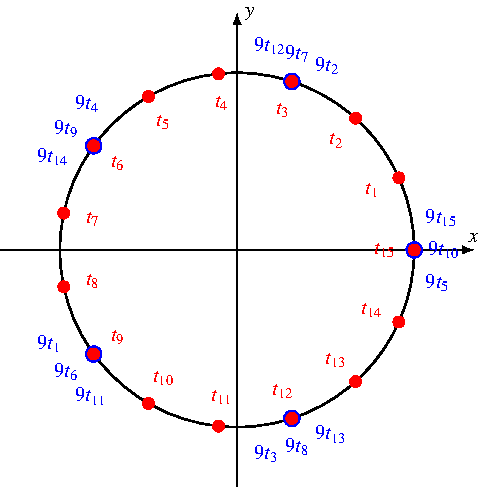
\includegraphics{chapters/6/trigosum.pdf}
\caption{Verteilung der Punkte $(\cos t_j, \sin t_j)$  auf dem Einheitskreis 
in rot.
Die Punkte $(\cos kt_j,\sin kt_j)$ für $k=9$ bilden eine Teilmenge, die
blau dargestellt ist.
Jeder blaue Punkt wird genau dreimal besucht, sie bilden ein gleichseitiges
Fünfeck mit den Punkten $(\cos 3t_j,\sin 3t_j)$ als Ecken.
Deren Schwerpunkt ist wieder der Nullpunkt.
\label{fourier:einheitskreis}
}
\end{figure}

\begin{satz}
\label{skript:fourier:orthogonalitaet1}
Ist $t_j=2\pi j/N$, dann gelten für beliebige ganze Zahlen $l$,
mit $0\le l\le n$, die Identitäten
\begin{equation*}
\begin{aligned}
\sum_{j=1}^N \cos lt_j
&=
\begin{cases}
N&\qquad l=0\\
0&\qquad\text{sonst}
\end{cases}
\\
\sum_{j=1}^N \sin lt_j
&=0.
\end{aligned}
\end{equation*}
\end{satz}

\begin{proof}[Beweis]
Wir betrachten zunächst den Fall $l=0$.
In diesem Fall ist $\cos lt_j=1$ und $\sin lt_j=0$ und damit
\[
\sum_{j=1}^N \cos lt_j = N
\qquad\text{und}\qquad
\sum_{j=1}^N \sin lt_j = 0.
\]
Im Folgenden können wir daher annehmen, dass $l\ne 0$.

In Abbildung~\eqref{fourier:einheitskreis} kann man sehen, dass die Punkte
$(\cos t_j,\sin t_j)$ auf dem Einheitskreis ein regelmässiges Polygon
mit $N$ Ecken bilden.
Der Schwerpunkt des Polygons ist ganz offensichtlich der Mittelpunkt.
Daraus folgt
\[
\sum_{j=1}^N \cos t_j = 0
\qquad\text{und}\qquad
\sum_{j=1}^N \sin t_j = 0.
\]
Damit ist der Satz für den Fall $l=1$ bewiesen.

Für beliebiges $l\ne 0$ beobachten wir, dass die Punkte 
$(\cos lt_j,\sin lt_j)$ eine Teilmenge der Punkte $(\cos t_j, \sin t_j)$
sind.
Wenn $l$ und $N$ teilerfremd sind, sind die Mengen gleich.
Wenn $l$ und $N$ dagegen den grössten gemeinsamen Teiler
$r=\operatorname{ggT}(l,N)$ haben, dann
ist die Menge 
\[
\{ 
(\cos lt_j,\sin lt_j)\,|\,j=1,\dots,N
\}
=
\{
(\cos rt_j,\sin rt_j)\,|\,j=1,\dots,N/r
\}
\]
ein regelmässiges Polygon mit $N/r$ Ecken.
Diese Situation ist in Abbildung~\ref{fourier:einheitskreis} mit den
blauen Punkten für den Fall $r=3=\operatorname{ggT}(9,15)$
illustriert.
Wie im Falle von $l=1$ folgt\footnote{Etwas formeller könnten wir sagen,
dass wir hier vollständige Induktion nach $N$ machen.
Was wir im letzten Schritt nämlich brauchen ist der Wert einer
trigonometrischen Summe mit $N/r<N$ Summanden, deren Werte wir gemäss
der naheligenden Induktionsannahme bereits kennen.},
dass der Schwerpunkt des Polygons der
Nullpunkt ist, und damit, dass
\begin{align*}
\sum_{j=1}^N \cos lt_j 
=
\sum_{j=1}^N \cos rt_j 
=
0,
\\
\sum_{j=1}^N \sin lt_j 
=
\sum_{j=1}^N \sin rt_j 
=
0.
\end{align*}
Damit ist alles gezeigt.
\end{proof}

In \eqref{fourier:produkte} werden die Summen von Produkten benötigt.
Mit üblichen trigonometrischen Umformungen kann man diese in Summen
von einfachen trigonometrischen Funktionen umwandeln.
Wir verwenden dazu die Formeln
\begin{align}
\cos\alpha\cos\beta
&=
\frac12\bigl(\cos(\alpha-\beta)+\cos(\alpha+\beta)\bigr),
\label{fourier:coscos}
\\
\sin\alpha\sin\beta
&=
\frac12\bigl(\cos(\alpha-\beta) + \cos(\alpha+\beta)\bigr).
\label{fourier:sinsin}
\\
\sin\alpha\cos\beta
&=
\frac12\bigl(\sin(\alpha-\beta) + \sin(\alpha+\beta)\bigr),
\label{fourier:sincos}
\end{align}
Damit können wir die Summen in \eqref{fourier:produkte} umwandeln:
\begin{align*}
\sum_{j=1}^N \cos kt_j\cos lt_j
&=
\sum_{j=1}^N \frac12\bigl(\cos (k-l)t_j +\cos(k+l)t_j\bigr)
\\
&=
\frac12\sum_{j=1}^N \cos (k-l)t_j
+ \frac12\underbrace{\sum_{j=1}^N\cos(k+l)t_j}_{\displaystyle=0}
\\
&=
\begin{cases}
\displaystyle\frac{N}2&\qquad k=l\\
0&\qquad\text{sonst}
\end{cases}
\\
\sum_{j=1}^N \sin kt_j \sin lt_j
&=
\sum_{j=1}^N \frac12\bigl(\cos(k-l)t_j +\cos(k+l)t_j\bigr)
\\
&=\frac12\sum_{j=1}^N \cos(k-l)t_j
+\frac12\underbrace{\sum_{j=1}^N \cos(k+l)t_j}_{\displaystyle=0}
\\
&=
\begin{cases}
\displaystyle\frac{N}2&\qquad k=l\\
0&\qquad\text{sonst}
\end{cases}
\\
\sum_{j=1}^N \sin kt_j \cos lt_j
&=
\sum_{j=1}^N \frac12\bigl(\sin(k-l)t_j +\sin(k+l)t_j\bigr)
\\
&=
\frac12\underbrace{\sum_{j=1}^N \sin(k-l)t_j}_{\displaystyle=0}
+
\frac12\underbrace{\sum_{j=1}^N \sin(k+l)t_j}_{\displaystyle=0}
=0.
\end{align*}
Damit haben wir den folgenden Satz bewiesen:

\begin{satz}
\label{skript:fourier:satzprodukte}
Für beliebige $k,l\in \mathbb N$ gilt
\begin{align*}
\sum_{j=1}^N
\cos kt_j \cos lt_j
&=
\begin{cases}
N                     &\qquad k=l=0\\
\displaystyle\frac{N}2&\qquad k=l > 0\\
0                     &\qquad\text{sonst}
\end{cases}
\\
\sum_{j=1}^N
\sin kt_j \sin l_j
&=
\begin{cases}
\displaystyle \frac{N}2&\qquad k=l\\
0                      &\qquad\text{sonst}
\end{cases}
\\
\sum_{j=1}^N
\sin kt_j \cos lt_j
&=
0
\end{align*}
\end{satz}
Mit dem Kronecker-$\delta$ 
\index{Kronecker-$\delta$}%
\[
\delta_{kl}
=
\begin{cases}
1&\qquad k=l\\
0&\qquad\text{sonst}
\end{cases}
\]
können wir die ersten zwei Formeln für $k,l>0$ noch etwas kompakter 
als
\begin{equation}
\sum_{j=1}^N
\cos kt_j \cos lt_j
=
\sum_{j=1}^N
\sin kt_j \sin l_j
=
\delta_{kl}\frac{N}2
\label{skript:fourier:trigsumsummary}
\end{equation}
schreiben.

In den folgenden Abschnitten verwenden wir diese Formeln, um die
Koeffizienten $a_k$ und $b_k$ zu bestimmen.
Der Koeffizient $a_0$ muss gesondert behandelt werden.

\subsection{Bestimmung von $a_0$}
In der Gleichung
\[
0
=
\sum_{j=1}^Ny_j
-Na_0
-\sum_{k=1}^na_k\underbrace{\sum_{j=1}^N\cos kt_j}_{\displaystyle=0}
-\sum_{k=1}^nb_k\underbrace{\sum_{j=1}^N\sin kt_j}_{\displaystyle=0}
\]
verschwinden die trigonometrischen Summen über $j$ nach
Satz~\ref{skript:fourier:orthogonalitaet1} und es bleibt die Gleichung
\begin{align*}
0
&=
\sum_{j=1}^Ny_j
-Na_0
\\
\Rightarrow\qquad
a_0&=\frac1{N}\sum_{j=1}^N y_j.
\end{align*}
Der Koeffizient $a_0$ ist der Mittelwert der Werte $y_j$.

\subsection{Bestimmung von $a_k, k>0$}
Zur Bestimmung von $a_k$ mit $k>0$ müssen wir die Gleichung
\[
0
=
\sum_{j=1}^N y_j\cos lt_j
-
a_0\underbrace{\sum_{j=1}^N\cos lt_j}_{\displaystyle=0}
-\sum_{k=1}^na_k\sum_{j=1}^N\cos kt_j\cos lt_j
-\underbrace{\sum_{k=1}^nb_k\sum_{j=1}^N\sin kt_j\cos lt_j}_{\displaystyle=0}
\]
heranziehen.
Die zweite und vierte Summe verschwindet wegen
Satz~\ref{skript:fourier:satzprodukte}, so dass wir die die Gleichung
\begin{align*}
0&=
\sum_{j=1}^N y_j\cos lt_j
-\sum_{k=1}^na_k\sum_{j=1}^N\cos kt_j\cos lt_j
\end{align*}
erhalten.
Die innere Summe über $j$ im zweiten Term verschwindet, wieder gemäss 
Satz~\ref{skript:fourier:satzprodukte}, für alle Werte
von $k$ ausser für $k=l$, in diesem Fall ist sie $N/2$. 
Damit können wir nach $a_k$ auflösen:
\begin{align*}
0&
=
\sum_{j=1}^N y_j\cos lt_j
-\sum_{k=1}^na_k\delta_{kl}\frac{N}2
=
\sum_{j=1}^N y_j\cos lt_j
-a_l\frac{N}2
\\
\Rightarrow\qquad 
a_l &= \frac{2}{N}\sum_{j=1}^Ny_j\cos lt_j.
\end{align*}

\subsection{Bestimmung von $b_k$}
Zur Bestimmung von $b_k$ müssen wir die Gleichung
\[
0=\sum_{j=1}^N y_j\sin lt_j 
-a_0\sum_{j=1}^N \sin lt_j
-\sum_{k=1}^na_k\sum_{j=1}^N\cos kt_j\sin lt_j
-\sum_{k=1}^nb_k\sum_{j=1}^N\sin kt_j\sin lt_j
\]
heranziehen.
Nach Satz~\ref{skript:fourier:satzprodukte}
verschwindet die zweite und die dritte Summe 
und in der letzten Summe
verschwinden alle Terme ausser der Term mit $k=l$, für den die
innere Summe über $j$ den Wert $N/2$ hat.
Damit wird die Gleichung vereinfacht zu
\begin{align*}
0
&=
\sum_{j=1}^Ny_j\sin lt_j - \sum_{k=1}^{n-1}b_l\delta_{kl}\frac{N}2
=
\sum_{j=1}^Ny_j\sin lt_j - b_l\frac{N}2
\\
\Rightarrow\qquad
b_l
&=
\frac{2}{N}\sum_{j=1}^Ny_j\sin lt_j.
\end{align*}

\subsection{Zusammenstellung der Resultate}
Sei $N=2n$ eine gerade natürliche Zahl.
Eine $2\pi$-periodische Funktion $f(t)$ kann als trigonometrisches Polynom
der Form
\[
p_n(t)
=
a_0 + \sum_{k=1}^{n-1} (a_k\cos kt + b_k\sin kt) + a_n\cos nt
\]
derart approximiert werden, dass zu den Zeiten $t_j=2\pi j/N, j=1,\dots,N$ 
die Funktion und das trigonometrische Polynom übereinstimmen:
\[
f(t_j) = y_j = p_n(t_j).
\]
Dazu müssen die Koefizienten
\begin{align*}
a_0
&=
\frac{1}N
\sum_{j=1}^N y_j,
\\
a_k
&=
\frac{2}N
\sum_{j=1}^N y_j\cos t_j
=
\frac{2}N
\sum_{j=1}^N y_j\cos \frac{2\pi j}{N}&\text{für }k&=1,\dots,n
\\
\text{und}\qquad
b_k
&=
\frac{2}N
\sum_{j=1}^N y_j\sin t_j
=
\frac{2}N
\sum_{j=1}^N y_j\sin \frac{2\pi j}{N}&\text{für }k&=1,\dots,n-1,
\end{align*}
verwendet werden.

\subsection{Beispiel: Dreiecksfunktion}
\begin{figure}
\centering
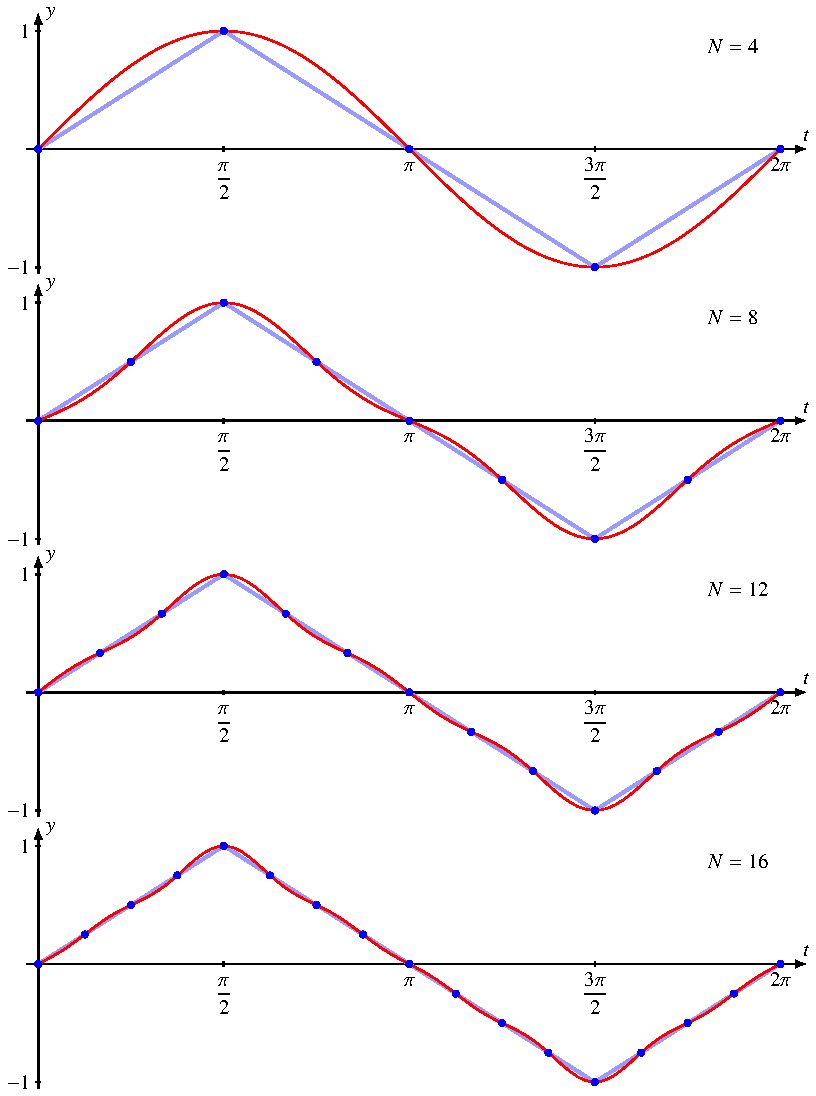
\includegraphics{chapters/6/dreieck.pdf}
\caption{Dreiecksfunktion ({\color{blue}blau}) approximiert mit
trigonometrischen Polynomen  $p_n(t)$ ({\color{red}rot})
mit verschiedenen Werten von $N=2n$.
\label{skript:fourier:beispiel}}
\end{figure}
\begin{table}
\centering
\setlength{\tabcolsep}{5pt}
\begin{tabular}{>{$}l<{$}>{$}r<{$}>{$}r<{$}>{$}r<{$}>{$}r<{$}>{$}r<{$}>{$}r<{$}>{$}r<{$}>{$}r<{$}}
&N=4&N=8&N=12&N=16&N=20&N=24&\dots&N=\infty\\
\hline
b_1&1& 0.85355& 0.82934& 0.82107& 0.81727& 0.81522&& 0.8105695\\
b_3& &-0.14645&-0.11111&-0.10124&-0.09704&-0.09484&&-0.0900633\\
b_5& &        & 0.05954& 0.04520& 0.04000& 0.03748&& 0.0324228\\
b_7& &        &        &-0.03249&-0.02519&-0.02207&&-0.0165422\\
b_9& &        &        &        & 0.02050& 0.01627&& 0.0100070\\
b_{11}&&      &        &        &        &-0.01413&&-0.0066989\\
%\hline
\end{tabular}
\caption{Nicht verschwindende Fourier-Koeffizienten der
Dreiecksfunktion~\eqref{skript:fourier:dreieck}
für verschiedene Werte von $N$.
In der Spalte ganz rechts unter $N=\infty$ die Werte für die
Fourierkoeffizienten der stetigen Fourier-Reihe
nach \eqref{fourier:normalekoeffizienten}.
\label{skript:fourier:dreieckkoef}}
\end{table}
Als Beispiel untersuchen wir die Approximation der
$2\pi$-periodischen Dreiecksfunktion, die auf dem Interval $[0,2\pi)$
durch
\begin{equation}
f(t)
=
\begin{cases}
\displaystyle t\cdot\frac{2}{\pi}    &\displaystyle \qquad 0\le t < \frac{\pi}2\\[8pt]
\displaystyle 2-t\cdot\frac{2}{\pi}  &\displaystyle \qquad \frac{\pi}2\le t < \frac{3\pi}2\\[8pt]
\displaystyle t\cdot\frac{2}{\pi} - 4&\displaystyle \qquad \frac{3\pi}2\le t <2\pi
\end{cases}
\label{skript:fourier:dreieck}
\end{equation}
gegeben ist,
mit Hilfe eines trigonometrischen Polynoms.
In Abbildung~\ref{skript:fourier:beispiel} ist die Dreiecksfunktion
hellblau dargestellt.

Weil die Funktion antisymmetrisch ist, verschwinden alle $a_k$-Koeffizienten.
Da die Funktion ausserdem symmetrisch ist bezüglich $\frac{\pi}2$ verschwinden
alle geraden $b_k$-Koeffizienten.
Für $N=4$ besteht $y$ nur aus vier Werten: $1$, $0$, $-1$ und $0$,
in diesem Fall muss die Funktion mit nur einem einzigen $\sin$-Term
mit dem Fourier-Koeffizienten $b_1$ darstellbar sein.
Tatsächlich ist $f(t) = \sin t$ an den Stellen $t_j=2\pi j/4$, $j=1,\dots,4$
(blau in Abbildung~\ref{skript:fourier:beispiel}),
dies wird in Abbildung~\ref{skript:fourier:beispiel} ganz oben gezeigt.
Erhöht man $N$, wird die Approximation immer besser, dies zeigen die
weiteren Graphiken in Abbildung~\ref{skript:fourier:beispiel}.

Die Berechnung der Fourier-Koeffizienten mit den Integralformeln
\eqref{fourier:normalekoeffizienten}
liefert für die Dreiecksfunktion~\eqref{skript:fourier:dreieck}
die Formel
\[
b_k = (-1)^{(k-1)/2}\frac{8}{\pi^2k^2}
\]
für ungereade Werte von $k$.
Diese Werte sind in der letzten Spalte unter $N=\infty$ dargestellt.
Für zunehmendes $N$ konvergieren die diskreten Koeffizienten $b_k$ gegen 
diese stetigen Werte.


%
% vektorgeometrie.tex
%
% (c) 2018 Prof Dr Andreas Müller, Hochschule Rapperswil
%
\section{Vektorgeometrische Interpretation}
\rhead{Vektorschreibweise}
Die bisherigen rein analytischen Betrachtungen verdecken den geometrischen
Gehalt der bisher entwickelten Theorie.
In diesem Abschnitt soll daher zunächst eine vektorielle Darstellung
aufgebaut, die dann erlauben soll, einerseits die Formeln für die 
Fourierkoeffizienten geometrisch zu verstehen und andererseits auf
komplexere Situationen zu verallgemeinern.

\subsection{Vektoren}
Die Operationen zur Bestimmung der Fourier-Koeffizienten können in 
vektorieller Schreibweise etwas übersichtlicher dargestellt werden.
Zunächst fassen wir die Funktionswerte $y_j$ in einem Vektor zusamen.
\begin{equation}
y = \begin{pmatrix}y_1\\\vdots\\y_N\end{pmatrix}
\end{equation}
Zur Berechnung der Fourier-Koeffizienten brauchen wir auch noch die
Werte der trigonometrischen Funktionen zu den Zeiten $t_j$, die wir
ebenfalls als Vektoren
\begin{align*}
c_0&=\begin{pmatrix}0\\\vdots\\0\end{pmatrix},
&
c_k&=\begin{pmatrix}\cos kt_1\\\vdots\\\cos kt_N\end{pmatrix},\;(k=1,\dots,n)
&&\text{und}
&
s_k&=\begin{pmatrix}\sin kt_1\\\vdots\\\sin kt_N\end{pmatrix},\;(k=1,\dots,n-1)
\end{align*}
schreiben.
Die Fourier-Koeffizienten können jetzt als Skalarprodukte geschrieben werden:
\begin{align*}
a_0 &=\frac1N c_0\cdot y,&
a_k &=\frac2N c_k\cdot y,\;(k=1,\dots,n),&
b_k &=\frac2N s_k\cdot y,\;(k=1,\dots,n-1).
\end{align*}

\subsubsection{Rekonstruktion der Funktion}
Auch die Darstellung der Funktion kann man wieder als Skalarprodukt schreiben.
Dazu schreiben wir die Fourier-Koeffizienten und die Werte der
trigonometrischen Funtionen also Vektoren
\begin{align*}
a
&=
\begin{pmatrix}
a_0\mathstrut\\
a_1\mathstrut\\
b_1\mathstrut\\
a_2\mathstrut\\
b_2\mathstrut\\
\vdots\\
b_{n-1}\mathstrut\\
a_n\mathstrut
\end{pmatrix}
&&\text{und}
&
e(t)
&=
\begin{pmatrix}
1\\
\cos t\\
\sin t\\
\cos2t\\
\sin2t\\
\vdots\\
\sin(n-1)t\\
\cos nt
\end{pmatrix}.
\end{align*}
Damit wird 
\[
p(t) = a\cdot e(t)
\]

\subsubsection{Orthogonalität}
Die Aussagen von Satz~\ref{skript:fourier:orthogonalitaet1}
lassen sich jetzt in geometrische Form fassen.
\begin{satz}
Es gilt
\begin{align*}
c_k\cdot c_l
&=
\begin{cases}
N&\qquad k=l=0\\
\displaystyle\frac{N}2&\qquad k=l>0\\
0&\qquad\text{sonst}
\end{cases}
\\
s_k\cdot s_l
&=
\begin{cases}
\displaystyle\frac{N}2&\qquad k=l\\
0&\qquad\text{sonst}
\end{cases}
\\
c_k\cdot s_l
&=
0
\end{align*}
\label{skript:fourier:orthogonalitaet}
\end{satz}

\begin{proof}[Beweis]
Die genannten Skalarprodukte sind nichts anderes als die Summen in
Satz~\ref{skript:fourier:orthogonalitaet1}:
\begin{align*}
c_k\cdot c_l
&=
\sum_{j=1}^N \cos kt_j \cos lt_j
=
\begin{cases}
N&\qquad k=l=0\\
\displaystyle\frac{N}2&\qquad k=l>0\\
0&\qquad\text{sonst}
\end{cases}
\end{align*}
und analog für die anderen Skalarprodukte.
Die Aussage des Satzes ist daher nichts anders als eine geometrische
Umformulierung der Aussagen des
Satzes~\ref{skript:fourier:orthogonalitaet1}.
\end{proof}

\subsubsection{Die Identität von Parseval}
Die Relationen von
Satz~\ref{skript:fourier:orthogonalitaet1}
besagen, dass die Vektoren $c_k$ und $s_k$ orthogonal sind.
Wir wenden Sie auf das Skalarprodukt der Funktion $f$ mit sich selbst an.
\begin{align*}
f\cdot f
&=
a_0^2 c_0\,\cdot c_0
+
\sum_{k=1}^na_k^2 \,c_k\cdot c_k
+
\sum_{k=1}^{n-1} b_k^2\,s_k\cdot s_k
\\
&=
Na_0^2
+
\frac{N}2\sum_{k=1}^n a_k^2
+
\frac{N}2\sum_{k=1}^{n-1} b_k^2
=
\frac{N}2
\biggl(
2a_0^2
+
\sum_{k=1}^n a_k^2
+
\sum_{k=1}^{n-1} b_k^2
\biggr)
\end{align*}
Damit haben wir den folgenden Satz bewiesen:
\begin{satz}[Parseval]
\[
\|f\|^2
=
\sum_{j=1}^N y_j^2
=
\frac{N}2
\biggl(
2a_0^2
+
\sum_{k=1}^n a_k^2
+
\sum_{k=1}^{n-1} b_k^2
\biggr)
\]
\end{satz}

\subsubsection{$2\pi$-Periodische Funktionen auf $\mathbb R$}
Die eben vektoriell dargestellte Analyse diskreter periodischer Funktionen 
kann verallgemeinert werden auf die Analyse von Funktionen auf
anderen Definitionsgebieten.
Benötigt wird eine Familie von Basisfunktionen und ein Skalarprodukt
$\langle\;,\;\rangle$ derart, dass die Basisfunktionen $g_i$ bezüglich
dieses Skalarproduktes orthonormiert sind, dass also
\[
\langle g_i,g_j\rangle
=
\delta_{ij}
=
\begin{cases}
1&\qquad i=j\\
0&\qquad\text{sonst}.
\end{cases}
\]
Jede Linearkombination
\[
f = \sum_{i} \alpha_i g_i
\]
von Basisfunktionen kann ebenfalls mit dem Skalarprodukt rekonstruiert
werden.
Dazu berechnet man
\[
\langle g_i,f\rangle
=
\biggl\langle
g_i,\sum_j\alpha_jg_j
\biggr\rangle
=
\sum_j \langle g_i,\alpha_jg_j\rangle
=
\sum_j \alpha_j\delta_{ij}
=
\alpha_i.
\]
Das Skalarprodukt kann auch verwendet werden, um einen Abstand zwischen
Vektoren als
\[
\| f-g\|^2
=
\langle f-g,f-g\rangle
\]
zu definieren.

Dieselbe Situation lässt sich auch für $2\pi$-periodische Funktionen 
auf $\mathbb R$ herbeiführen.
Als Basisfunktionen kann man die Funktionen 
\begin{equation}
\frac{1}{\sqrt{2}},\; \cos kx,\; \sin lx\quad k>0
\label{fourier:basis}
\end{equation}
verwenden.
Das Skalarprodukt $\langle f,g\rangle$ muss linear in $f$ und $g$ sein.
Eine naheliegende Wahl ist
\[
\langle f, g\rangle
=
\frac{1}{\pi}\int_{-\pi}^{\pi} f(x)\,g(x)\,dx.
\]
Wir überprüfen, ob die Funktionen orthogonal sind:
\begin{align*}
\left\langle \frac1{\sqrt{2}},\frac1{\sqrt{2}}\right\rangle
&=
\frac1{\pi}
\int_{-\pi}^{\pi} \frac12\,dx
=
1
\\
\left\langle \frac1{\sqrt{2}},\cos kx\right\rangle
&=
\frac1{\pi}\int_{-\pi}^{\pi}
\frac1{\sqrt{2}}\cos kx
\,dx
=0
\\
\left\langle \frac1{\sqrt{2}},\sin kx\right\rangle
&=
\frac1{\pi}\int_{-\pi}^{\pi}
\frac1{\sqrt{2}}\sin kx
\,dx
=0
\\
\langle \cos kx,\cos lx\rangle
&=
\frac1{\pi}
\int_{-\pi}^\pi \cos kx\cos lx\,dx
\\
&=
\frac1{\pi}
\int_{-\pi}^\pi
\frac12\bigl(
\cos (k-l)x+\cos (k+l)x
\bigr)
\,dx
=
\begin{cases}
1&\qquad k=l\\
0&\qquad\text{sonst}
\end{cases}
\\
\langle \sin kx,\sin lx\rangle
&=
\frac1{\pi}
\int_{-\pi}^\pi \sin kx\,\sin lx\,dx
\\
&=
\frac1{\pi}
\int_{-\pi}^\pi
\frac12
\bigl(
\cos (k-l)x - \cos (k+l)x
\bigr)
\,dx
=
\begin{cases}
1&\qquad k=l\\
0&\qquad\text{sonst}
\end{cases}
\\
\langle \sin kx,\cos lx\rangle
&=
\frac1{\pi}
\int_{-\pi}^{\pi} 
\frac12\bigl(
\sin (k-l)x + \sin (k+l)x
\bigr)
\,dx
=0
\end{align*}
Zu einer $2\pi$-periodischen Funktion $f(x)$ kann man daher immer
die Koeffizienten
\begin{equation}
\begin{aligned}
\bar{a}_0&=\frac1{\pi\sqrt{2}}\int_{-\pi}f(x)\,dx
\\
a_k&=\frac1{\pi}\int_{-\pi}^\pi f(x)\cos kx\,dx
\\
b_k&=\frac1{\pi}\int_{-\pi}^\pi f(x)\sin kx\,dx
\end{aligned}
\label{fourier:normalekoeffizienten}
\end{equation}
berechnen.
Die Linearkombination
\begin{equation}
\tilde f(x)
=
\bar{a}_0\cdot\frac1{\sqrt{2}}
+ 
\sum_{k=1}^\infty (a_k\cos kx+b_k\sin kx)
\label{fourier:reihe}
\end{equation}
ist natürlich wieder eine $2\pi$-periodische Funktion.

Ist $f(x)$ eine Linearkombination von Funktionen~\eqref{fourier:basis},
dann sind nur endlich viele der Koeffizienten $\bar{a}_0$, $a_k$ und $b_k$
sind von $0$ verschieden und es gilt $f(x)=\tilde f(x)$, die Summe
\eqref{fourier:reihe} rekonstriert die Funktion $f(x)$ also exakt..

Für eine beliebige $2\pi$-periodische Funktion $f(x)$ ist die Funktion
$\tilde f(x)$ nach \eqref{fourier:reihe} im Allgemeinen eine unendliche
Reihe.
Die Reihe \eqref{fourier:reihe} heisst die Fourier-Reihe der Funktion 
$f(x)$.
\index{Fourier-Reihe}

In der Literatur wird $a_0$ meistens anders definiert, nämlich als
\[
a_0 = \frac1{\pi}\int_{-\pi}^{\pi} f(x)\,dx = \sqrt{2}\bar{a}_0
\qquad\Rightarrow\qquad
\bar{a}_0 = \frac{a_0}{\sqrt{2}}
\]
Der erste Term der Reihe~\eqref{fourier:basis} wird dann
\[
\bar{a}_0\cdot\frac1{\sqrt{2}}
=
\frac{a_0}{\sqrt{2}}\cdot\frac{1}{\sqrt{2}}
=
\frac{a_0}2
\]
und die Fourier-Reihe ist
\begin{equation}
\tilde f(x)
=
\frac{a_0}2
+
\sum_{k=1}^\infty (a_k\cos kx+b_k\sin kx).
\end{equation}

\subsection{Fourier-Transformation}
Die Fourier-Koeffizienten $a_k$ und $b_k$ hängen linear von den
Funktionswerten $y_j$ ab.
Der Vektor der Fourier-Koeffizienten muss daher der Bildvektor des
Vektors $\vec y$ der Funktionswerte unter einer linearen Transformation
sein.
In diesem Abschnitt soll zunächst diese diskrete Fourier-Transformation 
hergeleitet werden.
Anschliessend soll gezeigt werden, wie sich diese Eigenschaft auf 
periodische Funktionen und auf beliebige Funktionen auf $\mathbb R$
ausdehenen lässt.

\subsubsection{Diskrete Fourier-Transformation}
Die Berechnung der Fourier-Koeffizienten ist eine lineare Operation
mit der $N\times N$-Matrix:
\[
A
=
\begin{pmatrix}
c_0^t\\
c_1^t\\
s_1^t\\
\vdots\\
c_{n-1}^t\\
s_{n-1}^t\\
c_n^t
\end{pmatrix}
=
\begin{pmatrix}
1           &1           &\dots &1            \\
\cos t_1    &\cos t_2    &\dots &\cos t_N     \\
\sin t_1    &\sin t_2    &\dots &\sin t_N     \\
\cos 2t_1   &\cos 2t_2   &\dots &\cos 2t_N    \\
\sin 2t_1   &\sin 2t_2   &\dots &\sin 2t_N    \\
\vdots      &\vdots      &\ddots&\vdots       \\
\sin(n-1)t_1&\sin(n-1)t_2&\dots &\sin(n-1)t_N \\
\cos nt_1   &\cos nt_2   &\dots &\cos nt_N    
\end{pmatrix}
\]
Die Orthogonalitätsrelationen von
Satz~\ref{skript:fourier:orthogonalitaet}
können jetzt neu geschrieben werden:
\begin{align*}
AA^t
&=
\begin{pmatrix}
c_0\cdot c_0&
	c_0\cdot c_1&
		c_0\cdot s_1&
			\dots&
				c_0\cdot c_{n-1}&
					c_0\cdot s_{n-1}&
						c_0\cdot c_n\\
c_1\cdot c_0&
	c_1\cdot c_1&
		c_1\cdot s_1&
			\dots&
				c_1\cdot c_{n-1}&
					c_1\cdot s_{n-1}&
						c_1\cdot c_n\\
s_1\cdot c_0&
	s_1\cdot c_1&
		s_1\cdot s_1&
			\dots&
				s_1\cdot c_{n-1}&
					s_1\cdot s_{n-1}&
						s_1\cdot c_n\\
\vdots	&\vdots	&\vdots	&\ddots	&\vdots	&\vdots	&\vdots	\\
c_{n-1}\cdot c_0&
	c_{n-1}\cdot c_1&
		c_{n-1}\cdot s_1&
			\dots&
				c_{n-1}\cdot c_{n-1}&
					c_{n-1}\cdot s_{n-1}&
						c_{n-1}\cdot c_n\\
s_{n-1}\cdot c_0&
	s_{n-1}\cdot c_1&
		s_{n-1}\cdot s_1&
			\dots&
				s_{n-1}\cdot c_{n-1}&
					s_{n-1}\cdot s_{n-1}&
						s_{n-1}\cdot c_n\\
c_n\cdot c_0&
	c_n\cdot c_1&
		c_n\cdot s_1&
			\dots&
				c_n\cdot c_{n-1}&
					c_n\cdot s_{n-1}&
						c_n\cdot c_n\\
\end{pmatrix}
\\
&=
\begin{pmatrix}
N     &0        &0        &\dots    &0        &0        &0        \\
0     &\frac{N}2&0        &\dots    &0        &0        &0        \\
0     &0        &\frac{N}2&\dots    &0        &0        &0        \\
\vdots&\vdots   &\vdots   &\ddots   &\vdots   &\vdots   &\vdots   \\
0     &0        &0        &\dots    &\frac{N}2&0        &0        \\
0     &0        &0        &\dots    &0        &\frac{N}2&0        \\
0     &0        &0        &\dots    &0        &0        &\frac{N}2
\end{pmatrix}.
\end{align*}
Bis auf die Faktoren $N$ und $\frac{N}2$ auf der Diagonalen ist
${\cal F}{\cal F}^t$ 
eine Diagonalmatrix.
Wir können die Matrix zu einer Einheitsmatrix machen, indem wir 
sie mit der Diagonalmatrix
\begin{equation}
D
=
\begin{pmatrix}
\sqrt{\frac1N}&0&\dots&0\\
0&\sqrt{\frac{2}{N}}&\dots&0\\
\vdots&\vdots&\ddots&\vdots\\
0&0&\dots&\sqrt{\frac{2}{N}}
\end{pmatrix}
\end{equation}
multiplizieren.
Wir schreiben
\begin{align*}
{\cal F}
&=
D\, A
\end{align*}
Wir nennen $\cal F$ die {\em Fourier-Matrix}.
\index{Fourier-Matrix}%
Die Fourier-Matrix $\cal F$ ist orthogonal, es gilt
\[
{\cal F}{\cal F}^t
=
DAA^tD^t
=
DD^tAA^t
=
E,
\]
wobei wir im letzten Schritt $D^t$ mit $AA^t$ vertauschen durften,
weil beide Diagonalmatrizen sind und damit vertauschen.
Insbesondere erhält $\cal F$ das Skalarprodukt, womit wir natürlich
nur die Parseval-Identität anders formuliert haben.

%
% komplex.tex
%
% (c) 2018 Prof Dr Andreas Müller, Hochschule Rapperswil
%
\subsubsection{Komplexe Fouriertransformation}
Bisher wurden alle Rechnungen nur mit reellen Zahlen durchgeführt.
Es stellt sich aber heraus, dass komplexe Zahlen für die Beschreibung
der Fourier-Transformation sehr viel praktischer sind.
Der Grund dafür ist die Eulersche Beziehung
\[
e^{it} = \cos t + i \sin t.
\]
und die Rechenregel
\[
e^{a+b}=e^a\cdot e^b
\qquad\Rightarrow\qquad
e^{ikt}=\cos kt+i\sin kt
\]
für die Exponentialfunktion.
Für die Fourier-Koeffizienten werden die Summen
\[
a_0
=
\frac{1}{N}\sum_{j=1}^N y_j,\qquad
a_l
=
\frac{2}{N}\sum_{j=1}^N y_j \cos lt_j,
\qquad\text{und}\qquad
b_l
=
\frac{2}{N}\sum_{j=1}^N y_j \sin lt_j
\]
benötigt.
Fassen wir $a_l$ und $b_l$ als Real- und Imaginärteil einer komplexen
Zahl auf, dann können wir 
\begin{align*}
c_l
=
a_l+ib_l
&=
\frac2{N} \sum_{j=1}^N y_j (\cos lt_j + i \sin lt_j)
=
\frac2{N} \sum_{j=1}^N y_j e^{lt_j}
\end{align*}
berechnen.

Auch die Rekonstruktion~\eqref{skript:fourier:rekonstruktion} ist
mit komplexen Zahlen darstellbar.
Dazu verwendet man 
\[
\cos kt = \operatorname{Re} e^{ikt}
\qquad\text{und}\qquad
\sin kt = \operatorname{Im} e^{ikt}.
\]
In dieser Form
\[
f(t)
=
a_0
+\sum_{k=1}^n (a_k \cos kt + b_k \sin kt)
\]






\subsubsection{Fast Fourier Transform}

\subsubsection{Fourier-Transformation von $2\pi$-periodischen Funktionen}

\subsubsection{Fourier-Transformation von Funktionen auf $\mathbb R$}








\section*{Übungen}
\begin{uebungsaufgaben}
\item
Betrachten Sie die Differentialgleichung
\begin{equation}
\frac{dx}{dt}
=
x^4-4x^2-\lambda
\label{aufgabe301:gl}
\end{equation}
\begin{teilaufgaben}
\item
Finden Sie die Gleichgewichtslösungen und untersuchen Sie die 
Bifurkationen, die bei Veränderungen des Parameters $\lambda$
auftreten können.
\item
Welche Gleichgewichtslösung wird das System einnehmen, wenn der
Parameter $\lambda$ erst von $-1$ auf $1$ anwächst
und dann wieder auf $-1$ absinkt.
\end{teilaufgaben}

\begin{loesung}
\begin{figure}
\centering
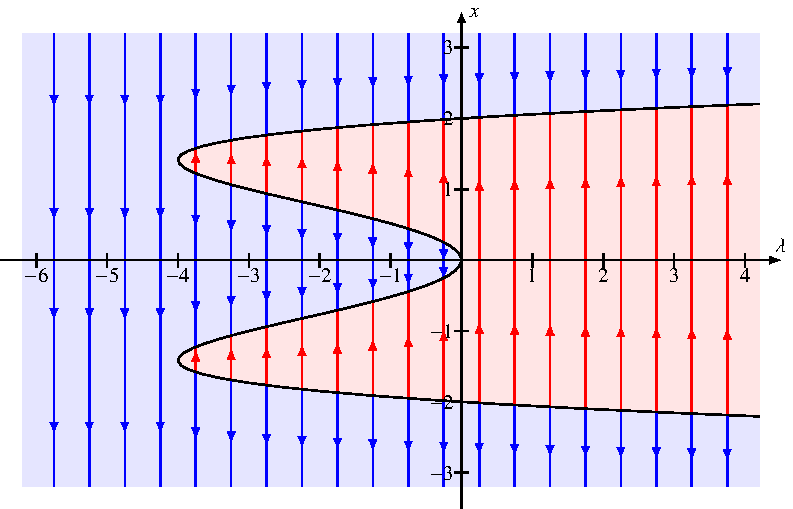
\includegraphics{chapters/3/grad4.pdf}
\caption{Phasendiagramm der Differentialgleichung~\eqref{aufgabe301:gl}.
\label{aufgabe301:fig}}
\end{figure}
\begin{teilaufgaben}
\item
Die kritischen Punkte der Differentialgleichung~\eqref{aufgabe301:gl}
sind Nullstellen der Gleichung
\begin{equation}
x^4-4x^2-\lambda=0
\label{aufgabe301:nullstellen}
\end{equation}
Dies ist eine quadratische Gleichung in $x^2$, die mit der Lösungsformel
für die quadratische Gleichung gelöst werden kann:
\[
x^2 = 2 \pm \sqrt{4+\lambda}.
\]
Diese Gleichung hat reelle Lösungen für $\lambda \ge -4$.
Für $\lambda \le 0$ ist die Quadratwurzel nicht grösser als $2$,
so dass die beiden Nullstellen positiv sind, es also vier verschiedene
Lösungen
\begin{equation}
x_{1,2,3,4} = \pm\sqrt{2\pm\sqrt{4+\lambda}}
\end{equation}
hat.
Für $\lambda >0$ hat die quadratische Gleichung eine negative Lösung
für $x^2$, die also nicht zu einer reellen Lösung der
Gleichung~\eqref{aufgabe301:nullstellen} führen kann.
Nur aus der positive Lösung $2+\sqrt{4+\lambda}$ kann man eine
Gleichgweichslösung, nämlich
\[
x=\pm\sqrt{2+\sqrt{4+\lambda}}
\]
ableiten.
Für $\lambda < -4$ gibt es gar keine Gleichgewichtslösung.

Das Phasendiagramm in Abbildung~\ref{aufgabe301:fig} zeigt,
dass für $\lambda >0$ die obere Gleichgewichtslösung stabil ist,
untere dagegen instabil.
Für $-4\le\lambda\le 0$ sind die Gleichgewichtslösungen
\begin{align*}
&\sqrt{2+\sqrt{4+\lambda}}
&&\text{und}&
&-\sqrt{2-\sqrt{4+\lambda}}
\\
\intertext{stabil und die Gleichgewichtslösungen}
&-\sqrt{2+\sqrt{4+\lambda}}
&&\text{und}&
&\sqrt{2-\sqrt{4+\lambda}}
\end{align*}
instabil.

Bei $\lambda=-4$ finden gleichzeitig zwei Sattel-Knoten-Bifurkationen 
statt, bei $\lambda=0$ findet ein einfache Sattel-Knoten-Bifurkation
statt, jedoch in umgekehrter Richtung wie im Beispiel im Text.
\item
Beim Anwachsen des Parameters über den Punkt $\lambda=0$ springt die
Gleichgewichtslösung auf die stabile Lösung
\[
x(\lambda)=\sqrt{2+\sqrt{4+\lambda}}.
\]
Bei der anschliessenden Verringerung von $\lambda$ bleibt die 
Gleichgewichtslösung auf dem Ast $x(\lambda)$ der Kurve, da diese
alle stabil sind.
Unabhängig vom Ausgangszustand befindet sich das System am Ende des
beschriebenen Szenarios also immer in der Nähe der Gleichgewichtslösung
\[
x(-1)=\sqrt{2+\sqrt{3}}.
\qedhere
\]
\end{teilaufgaben}
\end{loesung}


\end{uebungsaufgaben}

